\documentclass[11pt,letterpaper]{article}

% Load some basic packages that are useful to have
% and that should be part of any LaTeX installation.
%
% be able to include figures
\usepackage{graphicx}
% get nice colors
\usepackage{xcolor}

% change default font to Palatino (looks nicer!)
\usepackage[latin1]{inputenc}
\usepackage{mathpazo}
\usepackage[T1]{fontenc}
% load some useful math symbols/fonts
\usepackage{latexsym,amsfonts,amsmath,amssymb}

% comfort package to easily set margins
\usepackage[top=1in, bottom=1in, left=1in, right=1in]{geometry}

% control some spacings
%
% spacing after a paragraph
\setlength{\parskip}{.15cm}
% indentation at the top of a new paragraph
\setlength{\parindent}{0.0cm}


\begin{document}

\begin{center}
\Large
Ay190 -- Worksheet 10\\
John Pharo\\
Date: \today\\
Browncoats: Anthony Alvarez
\end{center}

\section*{Problem 1}

Using the Forward Euler method and 100 points, we get the results

\[
\begin{array}{ccc}
\text{Iterations} & z_1 & \phi_1 \\
1 & 0.139995919541 & 7.56727111528e-10 \\
2 & 0.139995918784 & -1.38777878078e-16
\end{array}
\]

\begin{figure}[!htb]\centering
  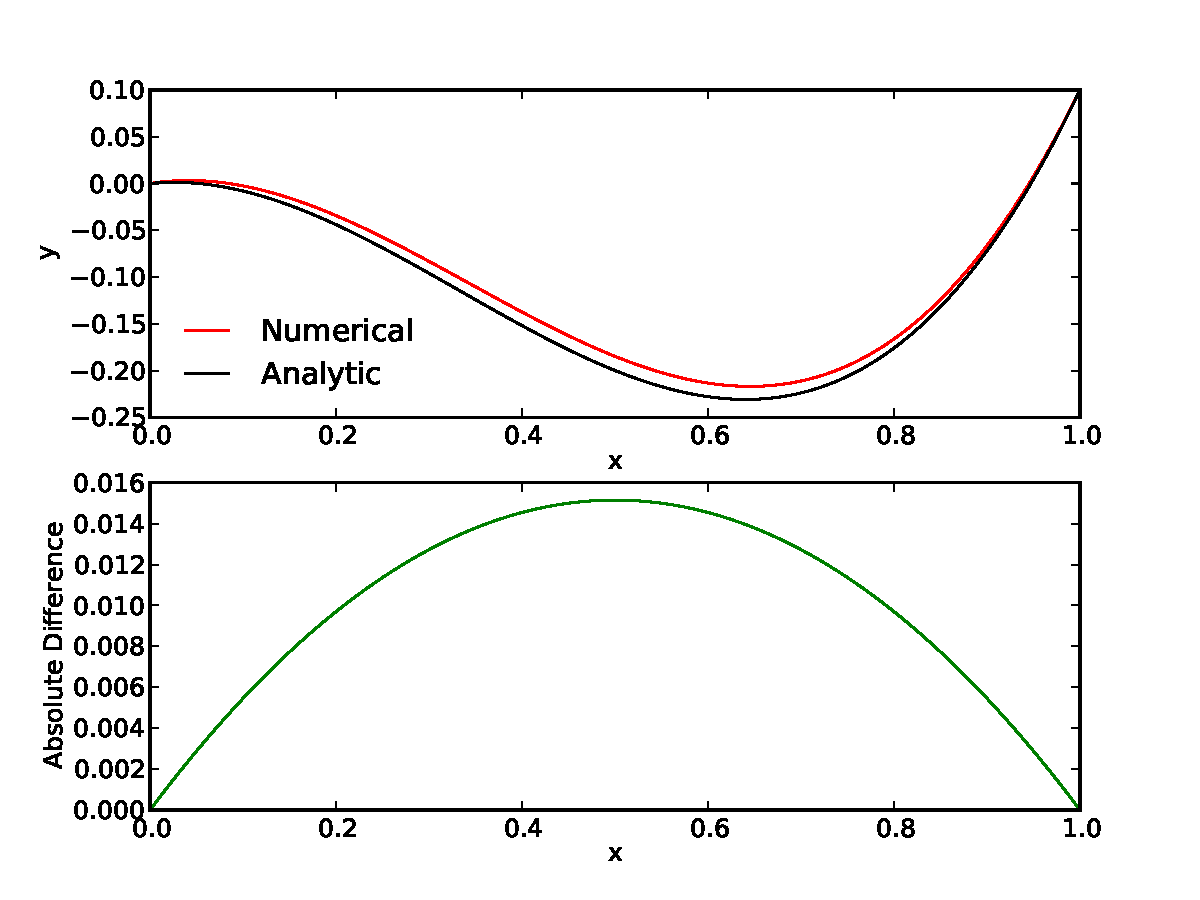
\includegraphics[width=1\textwidth]{BVP}
  \caption{Plot of the numerical and analytic solutions to the BVP using Forward Euler, along with a plot of the absolute difference between them, using 100 grid points.}
  \end{figure}

Using the RK2 method and 100 points, we get the results

\[
\begin{array}{ccc}
\text{Iterations} & z_1 & \phi_1 \\
1 & 0.109496466815 & -3.19267806637e-10 \\
2 & 0.109496467133 & -5.55111512313e-17 
\end{array}
\]

\begin{figure}[!htb]\centering
  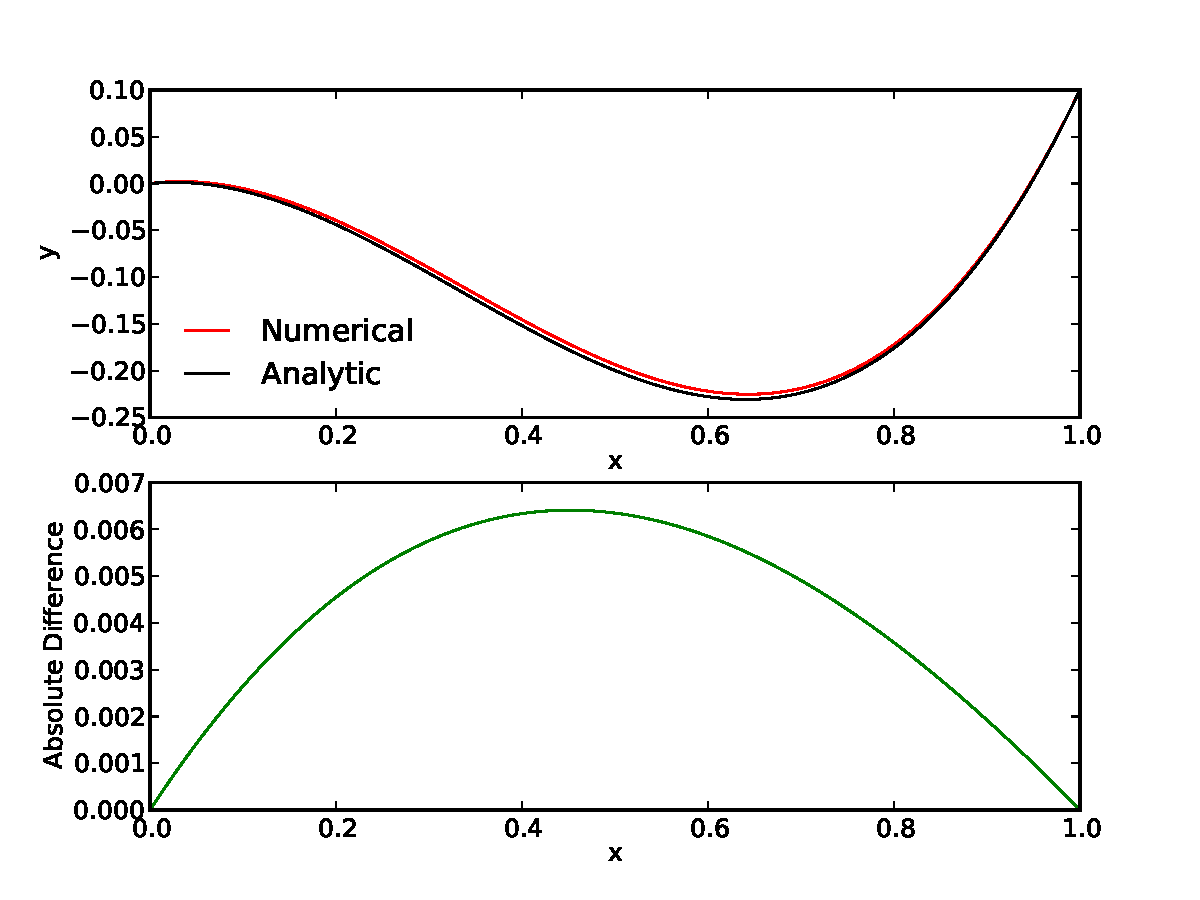
\includegraphics[width=1\textwidth]{BVP-RK}
  \caption{Plot of the numerical and analytic solutions to the BVP using RK2, along with a plot of the absolute difference between them, using 100 grid points.}
  \end{figure}

\begin{figure}[!htb]\centering
  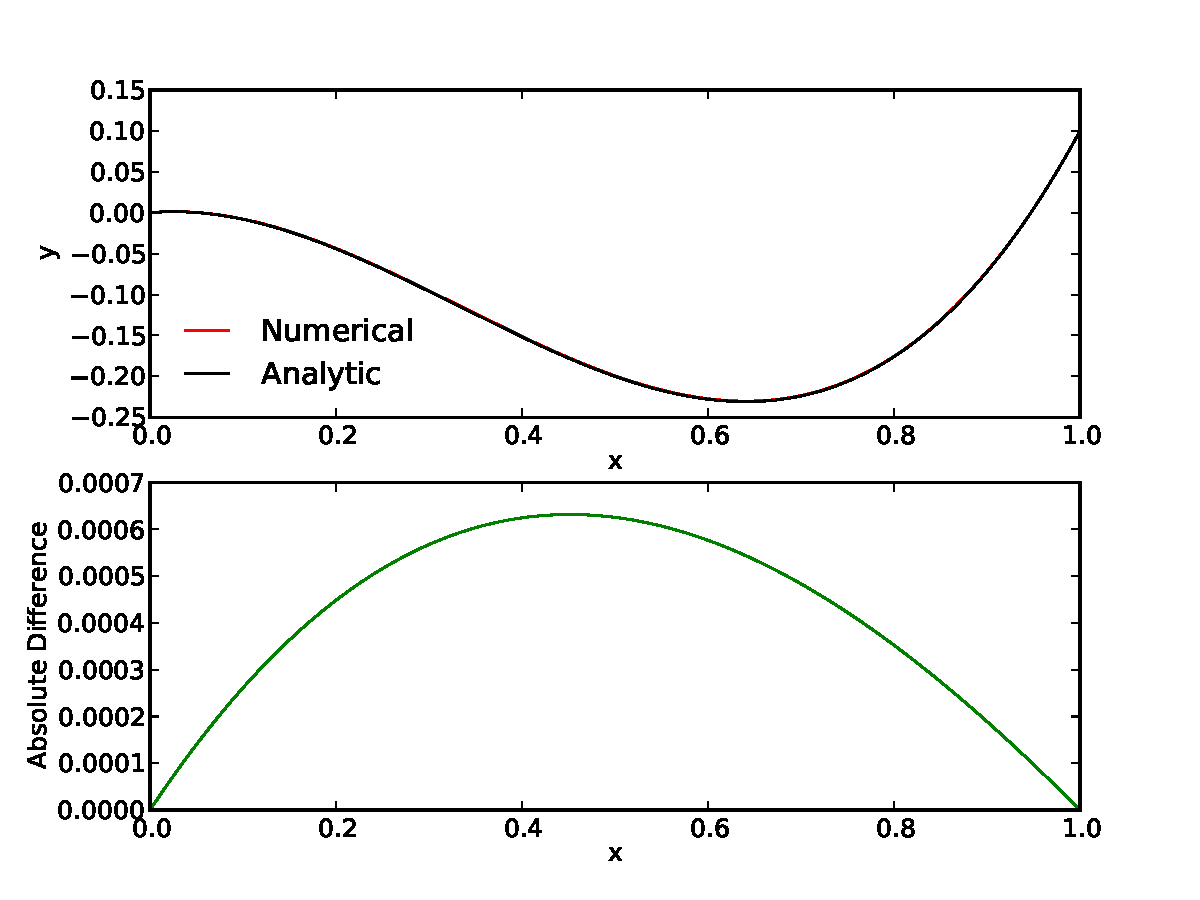
\includegraphics[width=1\textwidth]{BVP-RK2}
  \caption{Plot of the numerical and analytic solutions to the BVP using RK2, along with a plot of the absolute difference between them, using 1000 grid points.}
  \end{figure}

By changing the number of points used from 100 to 1000, and therefore decreasing the step size, the plots of the numerical and analytic solutions become basically visually indistinguishable. Furthermore, one can see from the difference plots that the differences decreased by a factor of 10, for a factor of 10 decrease in step size.

\end{document}
